\documentclass[12pt,a4paper,twocolumn]{article}

\usepackage[top=0.8in, left=0.6in, right=0.6in, bottom=0.8in]{geometry}
\usepackage{natbib}
\usepackage[hidelinks]{hyperref}

\usepackage{color}

\usepackage{graphicx}
\usepackage{caption}
\usepackage{subcaption}


\usepackage{multicol}
\usepackage{multirow}

\author{Dionisio Perez-Mavrogenis}
\title{{Technical Report : Feature Selection Challenge}}
	
\begin{document}

\maketitle
\section{Abstract}
This paper is concerned with investigating using filter methods for selecting optimal feature subsets from a large feature space for the purpose of binary classification. The feature selection by \citep{filter_svms} is implemented, confirming their results, and feature selection is also done using the Pearson criterion. Their performance is compared using SVM classification on the GISETTE and ARCENE datasets from the NIPS 2003 challenge and by the classification error of the test set, calculated by the competition evaluation system.

\section{Classification Method}
The paper investigated was \citep{filter_svms}. In particular, \citep{filter_svms} used Equation \ref{fisher_score} for determining each feature's relevance and then kept the best $N$ features, where $N$ was the number of features that minimized the training error of an SVM, as shown in Fig.~\ref{fig:no_features}. 

The SVM used in this paper is different than the one used by \citep{filter_svms},where a mixture of hard and soft-margin SVMs with a (modified) linear kernel was used. The SVM used in this paper was a soft-margin Gaussian kernel SVM as it was found to perform better. The value of $C$ and $\gamma$ was found by doing a grid-search with half of the features as described in \citep{grid_search}, using modified code from \citep{website:kitipat_heatmap}. The heat maps in Fig.~\ref{fig:heat_maps} show the optimal values for ARCENE and Fig.~\ref{fig:heat_maps_gisette} the values for GISETTE. The SVM library used was LIBSVM by \citep{libsvm}, as it was what \citep{filter_svms} used.

\begin{figure}
        \centering
        \begin{subfigure}[b]{0.5\textwidth}
                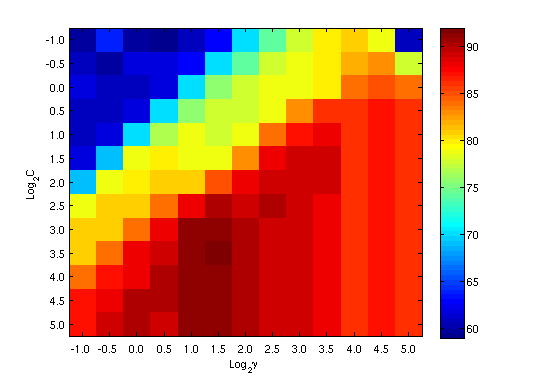
\includegraphics[width=\textwidth]{img/heat_map_huge_cv_10.png}
                \caption{Initial large heat map.}
                \label{fig:heat_map_large}
        \end{subfigure}
%        \begin{subfigure}[b]{0.55\textwidth}
%                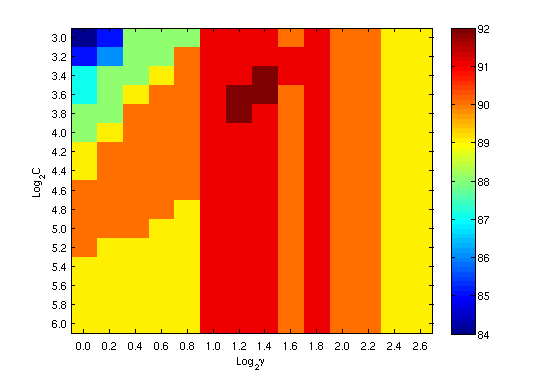
\includegraphics[width=\textwidth]{img/heat_map_medium_10cv.png}
%                \caption{Medium heat map.}
%                \label{fig:heat_map_med}
%        \end{subfigure}
        \begin{subfigure}[b]{0.5\textwidth}
           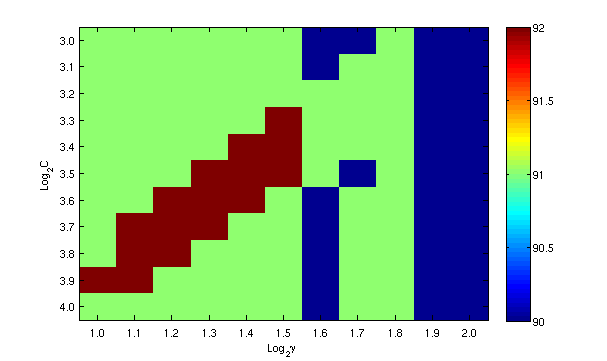
\includegraphics[width=\textwidth]{img/heat_map_small_cv_10.png}
           \caption{Small heat map.}
	 	   \label{fig:heat_map_small}
        \end{subfigure}
        \caption{{\footnotesize Heat maps for determining $C, \gamma$ for ARCENE. Optimals found are $C=2^{3.5}$ and $\gamma = 2^{1.5}$}}
        \label{fig:heat_maps}
\end{figure}

\begin{figure}
        \centering
        \begin{subfigure}[b]{0.4\textwidth}
                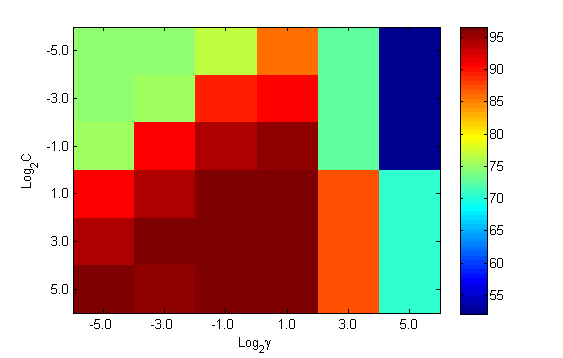
\includegraphics[width=\textwidth]{img/gisette_large.png}
                \caption{Initial large heat map.}
                \label{fig:heat_map_large}
        \end{subfigure}
        \begin{subfigure}[b]{0.4\textwidth}
                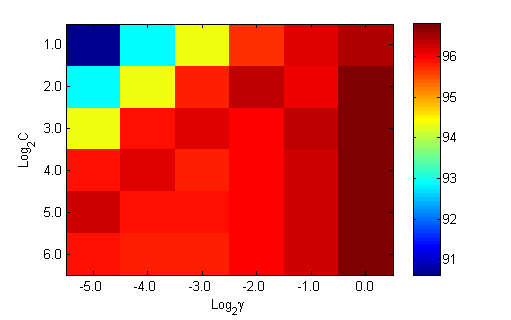
\includegraphics[width=\textwidth]{img/gisette_small.png}
                \caption{Small heat map.}
                \label{fig:heat_map_med}
        \end{subfigure}
	
        \caption{{\footnotesize Heat maps for determining $C, \gamma$ for GISETTE. Optimum found at $C=32$ and $\gamma =1$.}}
        \label{fig:heat_maps_gisette}
\end{figure}

\section{Introduction to Feature Selection}
Feature selection is the process of identifying relevant features from the complete feature set of a dataset and working with these instead, effectively reducing the dimensionality of the data. Usually high-dimensional feature spaces contain some redundancy, as it is likely that more than one of the observed variables will describe the same property of a system but from a different perspective. As outlined in \citep{feature_selection_intro} feature selection can be viewed as a form of noise reduction. By reducing data dimensionality one is more likely to identify relationships within the data as well as gain in terms of both computational performance (less volume of data to process) and predictive power of the classifier (removing redundancy decreases the likelihood of the classifier to over-fit the data). Furthermore one might also gain in storage space or cost and transfer times as they have to deal with a reduced amount of information.

Current feature selection methods are broadly split into \emph{filter methods}, \emph{embedded methods} and \emph{wrapper methods}\citep{feature_selection_intro}\citep{filter_methods}. Although these three techniques try to achieve the same goal, they  go about their objective in different ways. Methods \emph{wrapper} and \emph{filter} are mostly similar, with the key difference between them being their evaluation criterion. \emph{Wrapper} methods usually evaluate a subset's performance by measuring the performance of a learning machine, making them computationally expensive, whereas \emph{filter} methods use statistical means for evaluation. Both can use a variety of search strategies to construct a feature subset, including greedy addition or elimination of features to a working subset, various heuristic methods or exhaustive search. \emph{Embedded} methods lie somewhere between the aforementioned  methods in terms of computational requirements and are tightly coupled to a learning machine, being incorporated as part of that machine's learning process.

\section{Datasets Considered}
The datasets used in this paper are ARCENE and GISETTE. The ARCENE dataset is non-sparse and describes a binary classification problem with continuous input variables and no missing values, having approximately 50\% non-zero entries. GISETTE is also a binary classification problem with continuous input variables and no missing values, but is sparse with approximately 13\% of entries being non-zero. Sample statistics of the datasets are given in Table~\ref{tab:pattern_info} and Table~\ref{tab:feature_info}.

The data used in this paper was pre-processed as in \citep{filter_svms} by using Equation~\ref{normalization_equation} for rescaling the data so that variables with large values will not dominate over variables with smaller values\citep{feature_selection_intro}, for example when calculating the difference of two patterns as their Euclidean distance, as well as making the data comparable with each other\citep{feature_selection_intro}.

\begin{equation}
x_k \to \frac{x_k}{1/m\sum_k||x_k||^2} \quad \forall ~ x_k , ~k= 1,\dots,m
\label{normalization_equation}
\end{equation}

\begin{table}
\center
    \caption{{\footnotesize Pattern information for the datasets considered in this paper.}}
    \label{tab:pattern_info}
    \begin{tabular}{| c | c | c | c |}
	
    \hline
    ~      & Set        & Positive & Negative \\ \hline
    ~      & Training   & 44           & 56           \\ \hline
    ARCENE & Validation & 44           & 56           \\ \hline
    ~      & Test       & 310          & 390          \\ \hline
    ~      & Training          & 3000            & 3000            \\ \hline
    GISETTE      & Validation          & 500            &500            \\ \hline
    ~      & Test          & 3250            & 3250 \\ \hline
    \end{tabular}
\end{table}


\begin{table}
\center
    \caption{{\footnotesize Feature information for the datasets used in this paper.}}
    \label{tab:feature_info}
    \begin{tabular}{| c | c | c |}
 \hline
    Dataset & Real Features & Probes \\ \hline
    ARCENE  & 7000          & 3000   \\ \hline
    GISETTE      & 2500             & 2500      \\ \hline
    \end{tabular}
\end{table}


\section{Algorithms Used}

We will be using filter methods for selecting optimal subsets of features and in particular correlation based approaches, namely the Fisher score criterion as used in  \cite{filter_svms} and the Pearson correlation coefficient. The feature set is greedily constructed by adding the $k$ highest ranking features to the existing set and then evaluating its training error.

A feature's Fisher score is defined for feature $j$ as

\begin{equation}
 R_j(X) = \frac{(\mu_j(X^+) - \mu_j(X^-))^2}{V_j(X^+)+ V_j(X^-)}  , \quad  j=1,\dots ,n
 \label{fisher_score}
\end{equation}

with $X$ an observation matrix, $\mu_j(X^+)$ the mean of feature $j$ over the positive instances of $X$ (accordingly for $\mu_j(X^-)$) and $V_j(X^+)  = 1/m \sum_{i=1}^m (x_{m,j}^+ - \mu_j(X^+) )^2 $, $x^+ \in X^+$ and $x_{m,j}$ denoting feature $j$ of observation $m$. Fig.~\ref{fig:scatter_bar} shows the correlation coefficients for ARCENE and confirms that many features have correlation coefficients of zero, indicating potential irrelevance, further supported by data in Fig.~\ref{fig:no_features} where one sees the cross-validation error not improving after a given number of features, implying that there is redundancy in the data and hence it is possible to reduce the data dimensionality. Fig.~\ref{fig:arcene_n} suggests using 5201 features for ARCENE and Fig.~\ref{fig:gisette_n} suggests using 801 features for GISETTE.

The Pearson correlation coefficient is defined as for a feature $j$ as

\begin{equation}
PC(j) = \frac{|\sum_{i=1}^m (x_{i,j} - \bar{x}_j)(y_i-\bar{y})|}{\sqrt{\sum_{i=1}^m(x_{i,j}-\bar{x}_j)^2\sum_{i=1}^m(y_i-\bar{y})^2}}
\label{eq:pearson}
\end{equation}

with the bar notation indicating an average over index $i$ \citep{feature_selection_intro}. A non-negative Pearson correlation coefficient indicates linear dependence while a value of 0 indicates no correlation\citep{filter_methods}.

\begin{figure}
        \begin{subfigure}[b]{0.55\textwidth}
                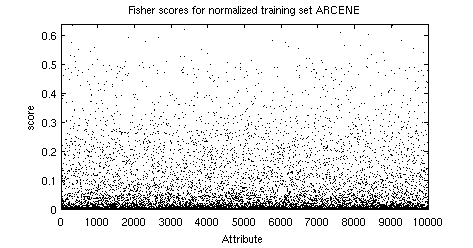
\includegraphics[width=\textwidth]{img/arcene_scatter.png}
                \caption{Correlation scores for each feature.},
                \label{fig:scatter}
        \end{subfigure}
        \begin{subfigure}[b]{0.55\textwidth}
                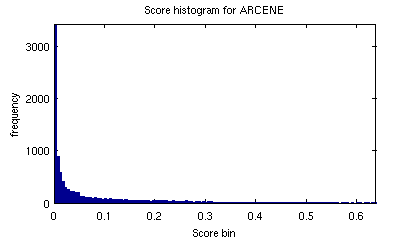
\includegraphics[width=\textwidth]{img/arcene_bar.png}
                \caption{Frequencies of correlation scores.}
                \label{fig:bar}
        \end{subfigure}
        \caption{{\footnotesize Frequencies of correlation scores for dataset ARCENE.}}
        \label{fig:scatter_bar}
\end{figure}

\begin{figure}
	\center
	\begin{subfigure}[b]{0.55\textwidth}
	        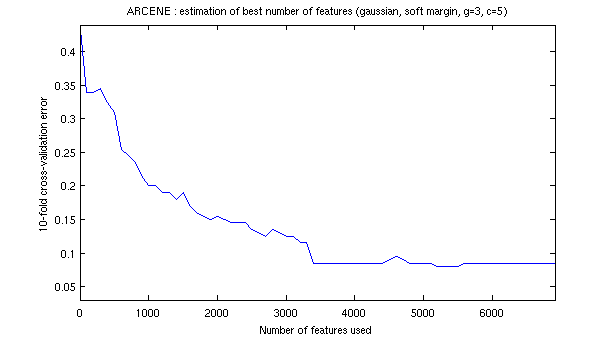
\includegraphics[width=\textwidth]{img/10f-cv.png}
			\caption{{\footnotesize ARCENE optimal value is 5201.}}
			\label{fig:arcene_n}
	\end{subfigure}
	
	\begin{subfigure}[b]{0.55\textwidth}
           	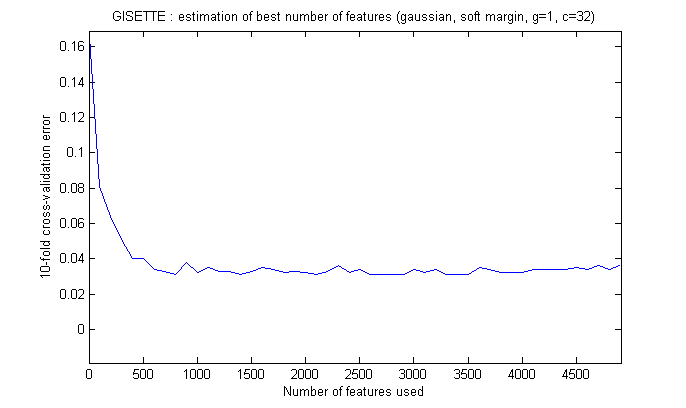
\includegraphics[width=\textwidth]{img/gisette_no_features.png}
	           \caption{{\footnotesize GISETTE optimal value is 801}.}
	           \label{fig:gisette_n}
        \end{subfigure}

        \caption{{\footnotesize10-fold cross validation for different number of features used. The features used were ranked by descending Fisher score.}}
        \label{fig:no_features}
\end{figure}



\begin{table*}
	\center
	\caption{{\footnotesize Performance of a Gaussian kernel SVM with Fisher scoring, trained on the validation and training sets for each dataset.A full set of information and submissions can be found at \protect\citep{website:competition_results}. }}

	\label{tab:arcene_results_all_data}

\begin{tabular}{|l|l|l|l|l|l|l|l|l|}
	\hline
	\multirow{2}{*}{Dataset}&\multicolumn{3}{|l|}{Balanced 	Error}&\multicolumn{3}{|l|}{Area Under Curve}&\multicolumn{2}{|l|}{Features}\\
	\cline{2-9}
	&Train&Valid&Test&Train&Valid&Test&\#&\%\\
	\hline
	arcene&0.0089&0.0114&0.1022&0.9821&0.9911&0.8978&5201&52.01\\
	\hline
	gisette &	0.0020 & 0.0020 &	0.0142	&0.9980	&0.9980	&0.9858&	801&	16.02 \\
	\hline
\end{tabular}

\begin{tabular}{|l|l|l|l|l|l|l|l|l|}
\hline
	\multirow{2}{*}{Dataset}&\multicolumn{3}{|l|}{Balanced 	Error}&\multicolumn{3}{|l|}{Area Under Curve}&\multicolumn{2}{|l|}{Features}\\
	\cline{2-9}
	&Train&Valid&Test&Train&Valid&Test&\#&\%\\
	\hline
arcene  & 0.0089     & 0         & 0.134     & 0.9911      & 1         & 0.866      & 5201         & 52.01         \\
\hline
gisette & 0.002      & 0.002     & 0.0166    & 0.998       & 0.998     & 0.9834     & 801          & 16.02        \\
\hline 
\end{tabular}
\end{table*}

\section{Discussion}

Several figures (Fig.~\ref{fig:scatter_bar}, Fig.~\ref{fig:arcene_n}) were recreated in this paper from \citep{filter_svms} in order to familiarize the author with the problem. While \citep{filter_svms} used both hard and soft-margin SVMs with a modified linear kernel, we used a Gaussian kernel soft-margin SVM for higher performance. This paper used univariate statistical methods, Fisher score and Pearson's correlation coefficients, for ranking features according to their relevance. The advantage of correlation based approaches is that they avoid the discretization of continuous variables, probability density estimation and are easy to implement\citep{filter_methods}. However it would be equally valid to consider multivariate relevance criteria, such as the RELIEF approach, which attempt to evaluate a feature's relevance in the context of other features\citep{feature_selection_intro}, perhaps aiding in feature creation.

Table~\ref{tab:arcene_results_all_data} presents the performance of an SVM trained  on the training and validation data and tested (by the NIPS system) on the outputs it produced for the testing data and one can see that the Pearson correlation coefficient performs slightly worse than the Fisher score. The Pearson coefficient is meaningful to use if there exists a linear relationship between the variables, in this case each feature's relationship with the resulting class. If the relationship is non-linear (which we don't know) then the index would fail to capture adequately the relationship, unless the  data is transformed \citep{garcia:correlation_tutorial}, and this might explain its inferior performance.

Filter methods implemented in this paper performed reasonably well, given the information they consider and their complexity and may be used effectively as a first approach to understanding the data at hand. Perhaps in a setting where making a false prediction is associated with a large loss on should consider a more powerful approach towards understanding the data.


\bibliographystyle{plainnat}
{\footnotesize	\bibliography{aml_cw2_report} }

\appendix

\section{Source Code Listing}
Some MATLAB code was developed for this coursework and a list of files with descriptions follows. Additionally, the LIBSVM \citep{libsvm} package was used for SVM classification and code for performing grid search by \citep{website:kitipat_heatmap}.

\begin{enumerate}
\item \texttt{initialize\_arcene.m} : Load data for ARCENE.
\item \texttt{initialize\_gisette.m}: Load data for GISETTE.
\item \texttt{main.m} Loads data and computes Fisher scores.
\item \texttt{normalize.m} Normalizes a data matrix as in \citep{filter_svms}.
\item \texttt{gisette\_num\_features.m} Select number of features for GISETTE.
\item \texttt{select\_num\_features.m} Select number of features for ARCENE.
\item \texttt{arcene\_train.m} Train and produce predictions for ARCENE.
\item \texttt{c\_graph.m} Explore what happens for various values of C.
\item \texttt{g\_c\_grid\_search.m} Modified grid search code from  \citep{website:kitipat_heatmap}.
\item \texttt{pearson\_test.m} Calculate the Pearson coefficients, train and test for all datasets.
\item \texttt{fisher\_relevance.m} Computes the Fisher score of the data matrix.
\item \texttt{train\_and\_test.m} Train and test an SVM on the input data. Also produces result files for submission.



\end{enumerate}
\end{document}
